%%
%% Toolbox Language Manual
%% $Id: roselink_man.tex,v 1.22 2006/04/19 10:25:20 vdmtools Exp $
%% 

%%%%%%%%%%%%%%%%%%%%%%%%%%%%%%%%%%%%%%%%
% PDF compatibility code. 

\makeatletter
\newif\ifpdflatex@
\ifx\pdftexversion\@undefined
\pdflatex@false
%\message{Not using pdf}
\else
\pdflatex@true
%\message{Using pdf}
\fi

\newcommand{\latexpdf}[2]{
  \ifpdflatex@ #1
  \else #2
  \fi
}

\newcommand{\latexorpdf}[2]{
  \ifpdflatex@ #2
  \else #1
  \fi
}

\makeatother

#ifdef A4Format
\newcommand{\pformat}{a4paper}
#endif A4Format
#ifdef LetterFormat
\newcommand{\pformat}{letterpaper}
#endif LetterFormat

%%%%%%%%%%%%%%%%%%%%%%%%%%%%%%%%%%%%%%%%

\latexorpdf{
\documentclass[\pformat,12pt]{article}
}{
% pdftex option is used by graphic[sx],hyperref,toolbox.sty
\documentclass[\pformat,pdftex,12pt]{article}
}

\usepackage[dvipdfmx]{graphicx, color}
\usepackage[dvipdfm,bookmarks=true,bookmarksnumbered=true,colorlinks,plainpages=true]{hyperref}

\usepackage{toolbox}
\usepackage{vdmsl-2e}
\usepackage{makeidx}
\usepackage{alltt}
\usepackage{here}

\usepackage{longtable}
\usepackage{ifthen}
\usepackage{verbatimfiles}


\usepackage{vpp}

\parindent0mm

\graphicspath{{figures/}}
\def\seename{$\Rightarrow$}

\newcommand{\vdmpp}{VDM++}
\newcommand{\vdmppEm}{VDM\/++}
\newcommand{\ToolboxName}{\vdmpp{} Toolbox}
\newcommand{\Toolbox}{Toolbox}
\newcommand{\link}{Rose-\vdmpp{} Link}
\newcommand{\rose}{Rose 98/2000}

\newcommand{\guicmd}[1]{{\sf #1}}
 
\makeindex
 
\begin{document}
\vdmtoolsmanualcsk{The Rose-VDM++ Link}
       {v9.0.6 beta}
       {2016}
       {VDM++}
       {1.2}

%%\nolinenumbering
%%\setindent{outer}{\parindent}
%%\setindent{inner}{0.0em}
%%\renewcommand{\thepage}{\roman{page}}

%%\label{endtofc}
%%\ifthenelse{\isodd{\pageref{endtofc}}}{\mbox{}\newpage}{}
%%\renewcommand{\thepage}{\arabic{page}}
%%\setcounter{page}{1}

%%\parskip2mm

\section{Introduction}
\label{intro}

Object-oriented analysis and design is a development method widely
used in the software engineering community. The {\it Unified Modelling
  Language (UML)} is a standard graphical language for expressing and
communicating object-oriented designs. UML was developed jointly by
Grady Booch, Ivar Jacobson, and Jim Rumbaugh at Rational Software
Corporation, with contributions from other leading methodologists,
software vendors, and many users. Being a merge of the Booch, OMT, and
Jacobson notations, the UML provides ways for business process,
object, and component modelling. Currently, several commercial CASE
tools support UML, one of which is Rose 2000, the successor to Rose 98
from Rational Software Corporation. Throughout the rest of this
document we refer to the two collectively as \rose{}.

Though well suited for the overall object-oriented design, UML is not
suited for giving formal semantics to the model. \vdmpp{}, on the
other hand, is designed for formal specification of object-oriented
systems with concurrent and real-time behaviour. The language is based
on ISO VDM-SL, and has been extended with class and object concepts,
facilitating the development of object-oriented formal specifications.

The {\it \link{}} combines the two languages. By defining and
implementing mapping rules between the two languages, the \link{}
allows the user to translate (parts of) a model represented in
\vdmpp{} to UML, and vice versa. The \link{} supports round-trip
engineering, allowing the user to start modelling the overall
object-oriented aspects of the system in UML, and proceed by giving
formal semantics to parts of the model by translating it to
\vdmpp{}. Subsequently the \vdmpp{} specification can be mapped, or merged,
back into UML, either for documentation purposes or
for further modelling of the object-oriented aspects of the
model. This mapping back and forth between the two representations can
continue until the model eventually is completed.

\subsubsection*{The \link{} - an Add-In to \rose{}}
The \link{} is installed as an Add-In to \rose{}, and it can be
activated or deactivated through the Add-In Manager of \rose{}. For
details on how to install the \link{} see \cite{InstallPPMan-CSK}.

\subsubsection*{Using This Manual}

This document is an extension to the {\it VDMTools User Manual (\vdmpp{})} \cite{UserManPP-CSK}.

Before continuing reading this
document it is recommended to read the Toolbox manual.
Moreover, knowledge about {\it UML} \cite{Booch&97} and \rose{} 
\cite{Rational98} is also preferable.

This manual is structured in the following way:

Section~\ref{roselink} describes the different features of the
\link{}, and Section~\ref{rose98} presents some important features
of \rose{}. To fully understand how the \link{} translates from one
representation to the other, it is important to understand the mapping
rules applied. These rules are described in
Section~\ref{mapping}. These rules are the theoretical
foundations of the \link{}. You can use the \link{} without reading
this section, but in many cases knowing the applied transformation
rules, will make the use of the tool easier. The transformation rules
are summarised in Figure~\ref{tab:mapping} in appendix~\ref{rules}.

The presentation of the capabilities of the \link{} is, whenever
necessary, accompanied with user scenarios and various screen
dumps. Furthermore some of the features of \rose{} are described
when needed.
  
With the distribution of the Toolbox a specification of different
sorting algorithms is included. It will be used in the following to
describe the use of the \link{}.  The example is described in
\cite{SortExpp-CSK}

\newpage
\section{The Rose-VDM++ Link}
\label{roselink}

This section presents the various services offered by the \link{}.  

The \link{} interfaces the CASE tool, \rose{}, to construct and
display classes in UML, and to let you edit the model at UML
level and map the modified model to \vdmpp{}.

The use of the tool can be divided into three categories:  

\begin{description}
\item[Mapping from UML to \vdmpp{} ({\em Forward Engineering}):] Use
  the \link{} to generate a \vdmpp{} specification from the classes
  defined in UML.
  
\item[Mapping from \vdmpp{} to UML ({\em Reverse Engineering}):] Will
  create a UML model from an existing \vdmpp{} specification.
  
\item[Synchronising UML and \vdmpp{} models:] During system
  development it is very likely that the \vdmpp{} model and the UML
  model of the system will be modified simultaneously. The \link{}
  allows you to keep track of the changes made in each model, and to
  synchronise the two models by merging them into one and
  subsequently propagate the merged model to UML and \vdmpp{}.
\end{description}

The basis for the \link{} is the mapping rules described in
Section~\ref{mapping}. They state exactly how different constructs are
mapped between \vdmpp{} and UML. 

Moreover, Section~\ref{mapping} describes, which parts of \vdmpp{} and
UML are not included in the mapping rules. For instance, the bodies of
operations and functions are not mapped to UML when reverse
engineering \vdmpp{} specifications. Only the signatures of functions
and operations are translated to UML. This does not, however, imply
that the function and operation bodies are lost --- they are simply
not visible in the UML model. If the UML model is later translated to
\vdmpp{} the bodies of functions and operations will be preserved.

In the same way the \link{} will not alter parts of the UML model that
are not included in the mapping rules. For instance, the UML model can
be extended with use cases, deployment diagrams, state transition
diagrams, etc. Such parts will simply be left unchanged by the
\link{}.

To fully understand the possibilities and limitations of the \link{},
some knowledge of how the \vdmpp{} Toolbox and \rose{} are connected,
as well as the flow of information between the two tools is
useful. Section~\ref{architecture} presents such information.
Section~\ref{main} presents the graphical user interface of the
\link{}. In Sections~\ref{trans1}-\ref{merging} the functionality of
the \link{} is described in detail and the three different ways of
translating between \vdmpp{} and UML are presented.
   
\subsection{The Architecture of The Rose-VDM++ Link}
\label{architecture}  

The architecture of the \link{} is illustrated in
Figure~\ref{fig:architecture}.  The figure illustrates how the
\vdmpp{} Toolbox and \rose{} are connected as well as the flow of data
between the tools.

\begin{figure}[htb]
\begin{center}
\mbox{}
\resizebox{14cm}{!}{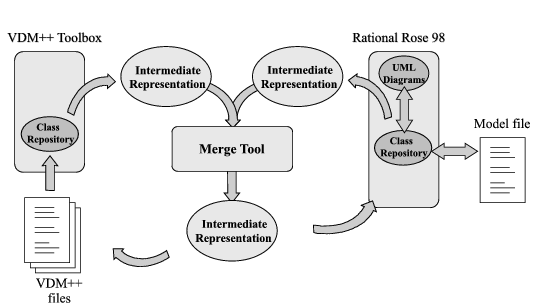
\includegraphics{vppuml_arch}}
\caption{The architecture of the \link{}.\label{fig:architecture}}
\end{center}
\end{figure}

Starting at the lower left corner of the figure, it shows how a set
of \vdmpp{} files (in {\tt rtf} format) are parsed and added to the class repository of
the \vdmpp{} Toolbox. The \link{} translates the \vdmpp{} specification
into an intermediate representation capturing the parts of \vdmpp{}
relevant in UML.

In the same way, by accessing the class repository of \rose{}, the UML
model is translated to the intermediate representation.

The two intermediate representations are ``compatible'' and can thus
be compared or merged. Merging the two models into one common model,
and subsequently propagate this model to the class repository in
\rose{} and the \vdmpp{} specification files, will synchronise the
\vdmpp{} and UML model.

The two representations can be merged in several different ways
resulting in the three ways of using the \link{}, described above.

If there is no intermediate representation resulting from \rose{} or
if one chooses to ignore such a representation, the merge will result
in a full translation from \vdmpp{} to UML.  Parallelly, if there is
no intermediate representation resulting from the \vdmpp{} Toolbox or
if one chooses to ignore such a representation, the result is a full
translation from UML to \vdmpp{}.  Finally, one can choose to merge
the two representations.

\subsection{The Main Rose-VDM++ Link Window}
\label{main}

This section describes the graphical user interface of the \link{}.

The \link{} is invoked from within the \vdmpp{} Toolbox by selecting the menu   
item {\it Tools/\link{}} or by pressing the 
\raisebox{-1.0mm}{
\includegraphics[width=0.03\textwidth]{rose}} 
(\guicmd{Rose}) button.

This is exactly the step shown in
Figure~\ref{fig:toolbox}.

\begin{figure}[htb]
\begin{center}
\mbox{}
\resizebox{9cm}{!}{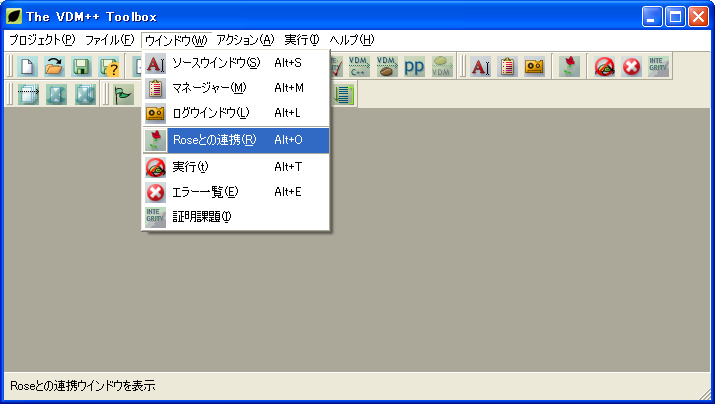
\includegraphics{invokeRose}}
\caption{Invoking the \link{}\label{fig:toolbox}}
\end{center}
\end{figure}

Invoking the \link{} opens a separate window as illustrated in Figure~\ref{fig:userinterface}.
While activated, all the features of the \link{} can be accessed from this window.  
The meaning of the different buttons will be described in the following sections.

\begin{figure}[htb]
\begin{center}
\mbox{}
\resizebox{9cm}{!}{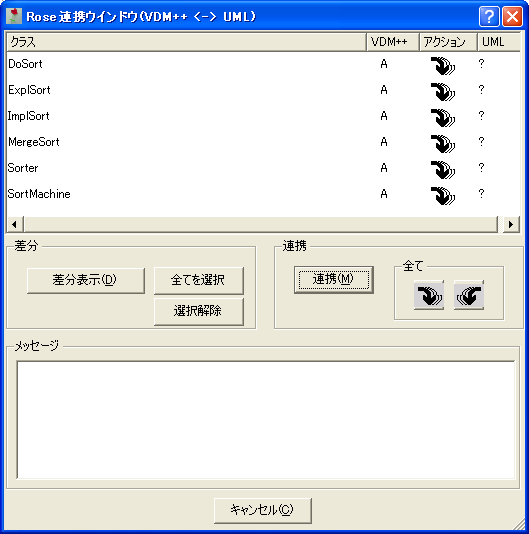
\includegraphics{roseWindow}}
\caption{The main window of the \link{}.\label{fig:userinterface}}
\end{center}
\end{figure}

When the \link{} is invoked, the necessary connection to \rose{} is
established. If an instance of \rose{} is already running on the
machine, the \vdmpp{} Toolbox connects to this instance. Otherwise
\rose{} is automatically started and a connection is established to
this instance. Subsequently the \link{} will read in a Rose Model File
following these simple rules:
\begin{itemize}
\item If the current project in the \ToolboxName{} is given a name
  (i.e.\ an existing project was opened or a new project was created
  and saved), the \link{} will try to open a model file with the same
  name and locataion as the project file. For example, for a project
  file {\tt MyProject.prj} the \link{} will open the model file
  {\tt MyProject.mdl} located in the same directory as the project file.
  If a model file with this name does not exist, an empty model file
  will be created.
\item If the current project in the \ToolboxName{} was never saved,
  the \link{} will simply use the model currently loaded into
  \rose{}.
\end{itemize}

% comment out by teramoto - using v7.2 or later, it isn't nessesary to use this fuction
% together with the \vdmpp{} project.

%It is recommended to use the \link{} together with a \vdmpp{} project
%file. The reason is that the \link{} will create all {\em new} files
%in the directory of the project file. Always using the \link{}
%together with a project file avoids that files are created in
%unexpected locations.

%comment out by teramoto end

When the \link{} is started the intermediate representations of the
\vdmpp{} and UML models are automatically computed, based on the
classes contained in the \vdmpp{} Toolbox and the classes contained in
\rose{}. The contents of the two representations are presented to the
user as a list of class names, with the state of each class in
\vdmpp{} and UML identified by designated status symbols. The exact
meaning of these symbols will be described in more detail later in
this section.
   
In the following sections we will describe how to translate one representation to the other   
as well as how to merge two representations using the \link{}. To illustrate the   
capabilities of the tool we will use the Sort Example of \cite{UserManPP-CSK}.  

\subsection{Translating VDM++ to UML}
\label{trans1}

If one or more classes have been syntax checked before the \link{} is
started, these classes are translated into the intermediate
representation using the mapping rules described in
Section~\ref{mapping}.  Assume now, that the \vdmpp{} Toolbox has been
configured for the files of the Sort Example and that a project file
with name {\tt Sortpp.prj} has been created. Assume furthermore, that
the \vdmpp{} files have been successfully syntax checked and that \rose{}
does not contain any class definitions. Invoking the \link{} would
then display a class list as shown in Figure~\ref{fig:VDMtoUML}.

\begin{figure}[htb]
\begin{center}
\mbox{}
\resizebox{9cm}{!}{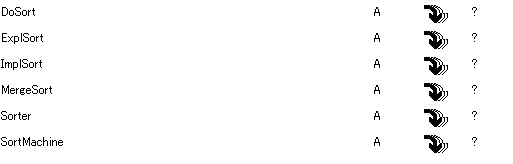
\includegraphics{sortClasses}}
\caption{The class list for the Sort example\label{fig:VDMtoUML}}
\end{center}
\end{figure}

The class designators used here are {\bf A} and  {\bf ?} with the
following meaning: 

\begin{description}  
\item [A]       Indicates that the class was added since the model was last computed.  
\item [?]       Indicates that the class is not known in this model.  
\end{description}  

Consequently the class list of Figure~\ref{fig:VDMtoUML} should be read as follows: All six classes have just   
been added to the \vdmpp{} model. On the other hand none of the classes defined in \vdmpp{}   
are known in the UML model, simply because we assumed that \rose{} did not contain   
any class definitions prior to invoking the \link{}.  

Each class in the list has its own action button used to configure how
the merge of the two representations should take place. When the
\link{} window is opened each button will be assigned a default
action, based on the two class designators of the associated class. To
change the state of an action button you simply click it. Each click
will toggle the state of the button between at most four different
states:

\begin{list}{}{}
\item[\resizebox{1cm}{!}{
\includegraphics{button1rosemanual}}] {\bf
    \vdmpp{} to UML:} This action will map the definitions of the
  class defined in \vdmpp{} to a class of the same name in UML. If
  this class exists in UML already it is updated. Otherwise a new
  class will be created.
\item[\resizebox{1cm}{!}{
\includegraphics{button2rosemanual}}] 
{\bf UML to \vdmpp{}:} This action will take the definitions of the class defined in   
  UML and map them to a class of the same name in \vdmpp{}. Consequently this will   
  create a new class or update the definitions of an already existing \vdmpp{} class   
  with the same name. See Section~\ref{trans2}.  
\item[\resizebox{1cm}{!}{
\includegraphics{button3rosemanual}}] 
{\bf Merge:} Selecting this action for a class will take the definitions of the class   
  defined in \vdmpp{} and merge them with the definitions of the class defined in UML.   
  See Section~\ref{merging}.  
\item[\resizebox{1cm}{!}{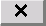
\includegraphics{button4rosemanual}}]
{\bf Exclude:} This will exclude the class from the new model being computed. As a   
  consequence the class will be removed from both the UML and \vdmpp{} model.    
\end{list}

In the example of Figure~\ref{fig:VDMtoUML} all action buttons are set
to map from \vdmpp{} to UML by default. Clicking one of the action
buttons will reveal that it is only possible to toggle between two
states, namely the ``\vdmpp{} to UML'' and the ``Exclude'' state. The
reason for this is that the other two possible states make no sense
since no classes are defined in \rose{}. If the state of the action
buttons have been changed, the default settings can be restored any
time by clicking the ``Default'' button.
  
And now back to the example: To make the \link{} perform the
translation from \vdmpp{} to UML, click the button labelled ``Map''.
The \link{} will now add six new classes to the class repository of
\rose{}.  All new classes generated by the \link{} are added to a
package named ``Generated classes''. At any time, however, a class may
be moved from the ``Generated classes'' package into another package.
If this class is later on being updated/modified by the \link{} it
will not be relocated to the ``Generated classes'' package.

Figure~\ref{fig:classrepository} shows a snapshot of the class
repository after having translated the \vdmpp{} classes of the Sort
Example to UML.

\begin{figure}[htb]
\begin{center}
\mbox{}
\resizebox{6cm}{!}{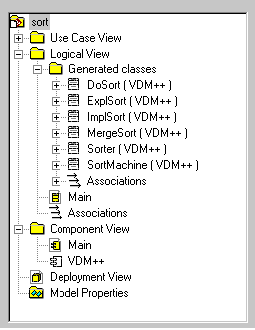
\includegraphics{classRepository}}
\caption{The class repository of \rose{} for the Sort example\label{fig:classrepository}}
\end{center}
\end{figure}

As an example, let us look at the UML class generated for the \vdmpp{}
class {\tt Sorter}. Figure~\ref{fig:SorterVDMUML} shows the
\vdmpp{} specification of the Sorter class and the generated UML
class. As you can see, the translation is very straightforward for
this class. For more information of the used mapping rules see
Section~\ref{mapping}.


\begin{figure}[htb]
\begin{center}
\hspace{-1.5cm}
%\begin{minipage}[t]{2in}
\resizebox{7cm}{!}{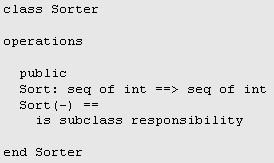
\includegraphics{sortervdm}}
%\end{minipage} \ \
%\begin{minipage}[t]{3in}
\hspace{0.2cm}
\resizebox{6cm}{!}{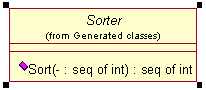
\includegraphics{sorteruml}}
%\end{minipage}
\caption{The \vdmpp{} {\tt Sorter} class (left) and the UML {\tt Sorter} class (right)\label{fig:SorterVDMUML}}
\end{center}
\end{figure}

In \rose{} you can browse the class repository
and inspect or modify the definitions of attributes and operations. Moreover you can create
class diagrams from the classes in the class repository.  
In Section~\ref{rose98} we will give a short introduction to \rose{}.

\subsubsection*{Generated Files}

Before updating the UML model of \rose{} the \link{} will create a
backup of the current UML model. The backup will be named by adding
{\tt \_old} to the name of the current model of \rose{}. For example
the model file {\tt MyProject.mdl} will backed up in {\tt
  MyProject\_old.mdl}. If the mapping from \vdmpp{} to UML presents
unexpected results, the changes made by the \link{} can easily be
undone from this backup.


\subsection{Translating UML to VDM++}
\label{trans2}
   
In this section we proceed by describing how to use the \link{} to
generate \vdmpp{} from a UML model defined in \rose{}.  To keep things
as simple as possible we will generate \vdmpp{} from the model
generated in Section~\ref{trans1}, and assume that the \vdmpp{}
Toolbox contains no model. I.e.\ we assume that there are no syntax
checked classes prior to the invocation of the \link{}. By selecting
the menu item {\it Project/New} of the \vdmpp{} Toolbox all previously
loaded classes from the \vdmpp{} Toolbox will be removed. 

% comment out by teramoto - using v7.2 or later, it isn't nessesary to use this fuction
% together with the \vdmpp{} project.

%Subsequently
%save this (empty) project to an empty directory and proceed with this
%example
%\footnote{The reason for saving the project even though no
%  files has been configured into it is to be able to control where new
%  files are created.}.

% comment out by teramoto end

Now, by selecting the menu item {\it Tools/\link{}}, the class list
shown in Figure~\ref{fig:UMLtoVDM} will be displayed. As expected, we
see that six classes are defined in UML whereas none of these classes
are known in \vdmpp{}.

\begin{figure}[htb]
\begin{center}
\mbox{}
\resizebox{9cm}{!}{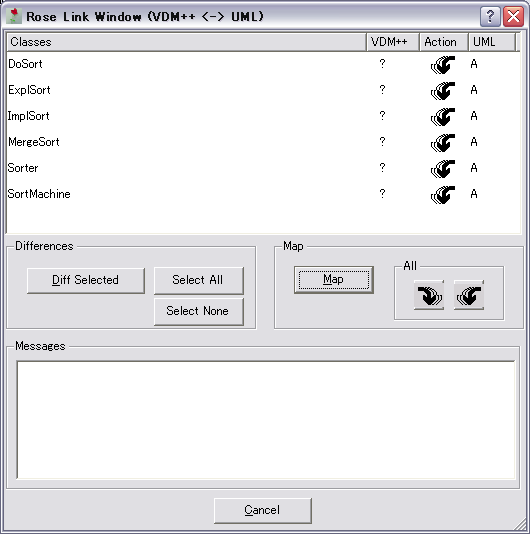
\includegraphics{classListUml}}
\caption{The class list for only UML classes\label{fig:UMLtoVDM}}
\end{center}
\end{figure}

Clicking the ``Map'' button now will display the dialog shown in Figure~\ref{fig:selectDirectory}.
You can select the directory to save the generated \vdmpp{} class files for the
six classes defined in UML.

\begin{figure}[!htb]
\begin{center}
\mbox{}
\resizebox{9cm}{!}{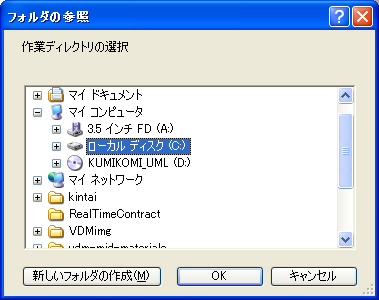
\includegraphics{seldir}}
\caption{The dialog to select directory for the generated \vdmpp{} classes \label{fig:selectDirectory}}
\end{center}
\end{figure}
As an example, Figure~\ref{fig:ExplSortVDMUML} shows the UML version of the class
{\tt ExplSort} and the \vdmpp{} specification generated for the same class. 
Notice that
the functions and operations are generated simply as signatures - the
user must specify the bodies of them later on.

\begin{figure}[htb]
\begin{center}
\mbox{}
\resizebox{6.5cm}{!}{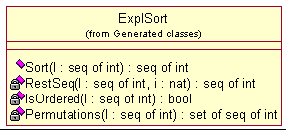
\includegraphics{explSortUml}}
\hspace{0.2cm}
\resizebox{7cm}{!}{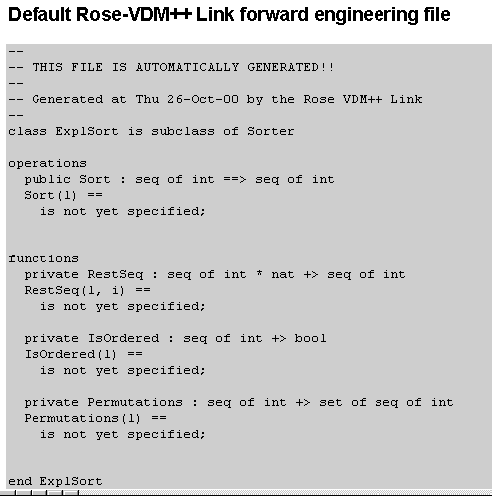
\includegraphics{explSortVdm}}
\caption{The UML {\tt ExplSort} class (left) and the \vdmpp{} {\tt ExplSort} class (right)\label{fig:ExplSortVDMUML}}
\end{center}
\end{figure}

\subsubsection*{Generated Files}

Each new class introduced in UML will be generated in a separate {\tt
  rtf} file with the same name as the class. For example the class
{\tt MyClass} will be generated to a file with the name {\tt
  MyClass.rtf} located in the same directory as the project file. If a
file with this name exists already, the \link{} issues a warning and
the new file will {\em not} be created. In this case the existing file
should be moved or renamed, or the class introduced in UML should be given
another name to avoid the name conflict.

The log window of the \vdmpp{} Toolbox will display the names of all
files generated, as well as the directory in which they were generated.

When generating new {\tt rtf} files for classes introduced in UML the
\link{} uses the special file named {\tt NewClass.rtf} as ``skeleton''
for the new file. This file {\em must} be located in the {\tt uml}
subdirectory of the \ToolboxName{} installation. The contents of this
skeleton file may be changed, but it is important that the following
requirements are met:
\begin{itemize}
\item The document should {\em always} contain a VDM block, i.e.\ at
  least one (possibly empty) paragraph in style {\tt VDM}.
\item The filename must be {\tt NewClass.rtf} and the file must be
  located in the {\tt uml} subdirectory of the \ToolboxName{} installation.
\end{itemize}


\subsubsection*{Using the Generated Classes}

The generated \vdmpp{} classes are automatically added to the current
project and parsed. This is possible, because the \link{} generates
classes which almost always will be syntax correct. However, it is
possible that syntax errors from the Rose model will be carried over
to the VDM++ model (normally inappropriate use of keywords).

You will now probably proceed by extending the \vdmpp{} specification,
for example by writing the bodies of operations and functions.  One
could also imagine, that you want to modify the object-oriented
aspects of the model (inheritance and association relations), or you
find it necessary to add new instance variables, functions, etc.

This should be done by simply editing the generated {\tt rtf} files.
Later, the new \vdmpp{} model can easily be reverse engineered to UML in order
to make the two models consistent. Syntax check the classes (and make
a type check if you like) and proceed as described in
Section~\ref{trans1}, provided that the UML model was not changed
during the modification of the \vdmpp{} model.

\subsubsection*{Warnings Generated during the Translation from UML to \vdmpp{}}

When a UML class is translated to \vdmpp{}, the UML attributes and
operations are converted to \vdmpp{} constructs.  The names and types
used in the UML model must consequently comply with the syntactical
rules of \vdmpp{}. If this is not the case, the UML definition is
simply ignored and the user is notified by a warning.  This is done in
order to maximise the syntactical correctness of the \vdmpp{}
specification generated.

It is important to give notice to the warnings generated when the
\link{} reads definitions from UML. The reason is that whenever a
warning is presented, something in the UML model could not be
translated to \vdmpp{}, and is consequently ignored in the common
representation being constructed. As a consequence of the architecture
of the \link{} (see Section~\ref{architecture}) the representation
computed by the Merge Tool will replace the current model in the class
repository of \rose{}. This means that constructs ignored while
reading the UML model are removed if the ``Map'' button is clicked!

See appendix~\ref{warnings} for more information.

\subsection{Merging VDM++ and UML Models}
\label{merging}

In Sections~\ref{trans1} and~\ref{trans2} we assumed that the model
was expressed in either \vdmpp{} or UML, i.e.\ one of the two 
representations of Figure~\ref{fig:architecture} was empty. This was
to keep matters as simple as possible, and to illustrate how it is
possible to take a model from one representation and translate it to
the other. This can be useful either when documenting an existing
\vdmpp{} specification by generating UML diagrams, or when generating
\vdmpp{} from an existing UML model. However, when modelling larger
and more complex systems, it is likely that the UML and \vdmpp{}
models will evolve simultaneously, and the assumption of
Sections~\ref{trans1} and ~\ref{trans2} do no longer hold. To meet
this requirement the \link{} facilitates the merging of two different
models into one, as will be described in this section.  

In the following we will assume that initially the \vdmpp{} Toolbox
has been configured with the Sort Example of Section~\ref{trans1}, and
that this specification has been translated to UML as described in
Section~\ref{trans1}. Subsequently, both the \vdmpp{} specification
and the UML model have been slightly modified.

Figure~\ref{fig:mergeUMLVDM} shows the class list of the \link{} after
some changes have been made to both the \vdmpp{} and the UML model.
\begin{figure}[htb]
\begin{center}
\mbox{}
\resizebox{9cm}{!}{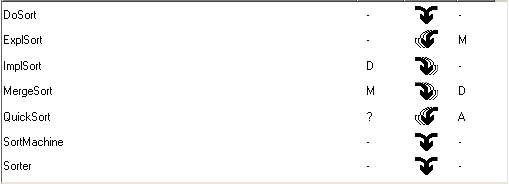
\includegraphics{bothChanged}}
\caption{Class list when both UML and \vdmpp{} have been changed\label{fig:mergeUMLVDM}}
\end{center}
\end{figure}
From this figure we can see that in UML a new class, {\tt QuickSort}
has been added and the class {\tt ExplSort} has been modified. Moreover, the
class {\tt MergeSort} has been removed from the model. In \vdmpp{} the
class {\tt MergeSort} has been modified and the class {\tt ImplSort} has been
deleted. 

Figure~\ref{fig:mergeUMLVDM} introduces three new class
designators {\bf M}, {\bf -} and {\bf D}, which together with the
previously mentioned two designators constitute the five different
class designators used in the \link{}. 

The three class designators have the following meaning:
\begin{description}  
\item [M] Indicates that the class was modified.  
\item [-] Indicates that the class has not changed.  
\item [D] Indicates that the class was deleted since the models were last computed.  
\end{description}  
To investigate the differences between two representations of the same
class, simply click the checkbox next to the class and subsequently
the ``Diff'' button. The result will be displayed in the log window.
To compute the differences of the \vdmpp{} and UML representations of
all classes, press the ``All'' button to select all classes.

Figure~\ref{fig:diffs} shows the result of computing the differences of
the \vdmpp{} and UML representations of all classes. We see, for example, that the
two versions of the {\tt ExplSort} class only differ in the name of one of the arguments to the
function {\tt RestSeq}; an ``{\tt i}''was changed to a ``{\tt j}''.

\begin{figure}[htb]
\begin{center}
\mbox{}
\resizebox{9cm}{!}{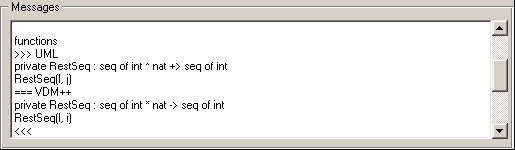
\includegraphics{differences}}
\caption{The differences between the \vdmpp{} and UML representations for all classes\label{fig:diffs}}
\end{center}
\end{figure}
Assume now, you want to merge these two models into one single
representation, which subsequently is propagated to the class
repository in \rose{} and the {\tt rtf} files containing the \vdmpp{}
specification.  

In order to determine how the merge of the two representations should
take place, the desired action has to be chosen by changing the states
of the action buttons. See Figure~\ref{tab:actions} for a list of
possible actions for the different classes.

\begin{figure}[ph]
\begin{center}
\mbox{}\vspace*{-1ex}
\begin{tabular}{|l|l|p{10cm}|} \hline
  Class            & Possible actions   & Consequences when pressing the ``Map'' button \\ \hline 
\hline
DoSort             & \resizebox{1cm}{!}{
\includegraphics{button3rosemanual}} (default)& No updates will be made, because the class has not been changed in either model.\\
                   & \resizebox{1cm}{!}{
\includegraphics{button1rosemanual}} & as the default action\\ 
                   & \resizebox{1cm}{!}{
\includegraphics{button2rosemanual}} & as the default action\\
                   & \resizebox{1cm}{!}{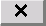
\includegraphics{button4rosemanual}} & The class will be excluded from both models.\\ \hline
Sorter             & \resizebox{1cm}{!}{
\includegraphics{button3rosemanual}} (default)& No updates will be made, because the class has not been changed in either model.\\
                   & \resizebox{1cm}{!}{
\includegraphics{button1rosemanual}} & as the default action\\ 
                   & \resizebox{1cm}{!}{
\includegraphics{button2rosemanual}} & as the default action\\
                   & \resizebox{1cm}{!}{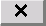
\includegraphics{button4rosemanual}} & The class will be excluded from both models.\\ \hline
ExplSort           & \resizebox{1cm}{!}{
\includegraphics{button2rosemanual}} (default) & The modification made in the UML model will also be made in the \vdmpp{} model.\\
                   & \resizebox{1cm}{!}{
\includegraphics{button1rosemanual}} & The modification previously made in the UML model will be deleted. The class returns to its previous state.\\ 
                   & \resizebox{1cm}{!}{
\includegraphics{button3rosemanual}} & A conflict will result, as explained below. \\
                   & \resizebox{1cm}{!}{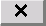
\includegraphics{button4rosemanual}} & The class will be excluded from both models.\\ \hline
ImplSort           & \resizebox{1cm}{!}{
\includegraphics{button1rosemanual}} (default) & The class will also be deleted from the UML model. \\ 
                   & \resizebox{1cm}{!}{
\includegraphics{button2rosemanual}} & A new ImplSort class will be generated in the \vdmpp{} model.\\
                   & \resizebox{1cm}{!}{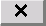
\includegraphics{button4rosemanual}} & as the default action\\ \hline
MergeSort           &
\resizebox{1cm}{!}{
\includegraphics{button1rosemanual}} (default) & A
new MergeSort class will be generated in the UML model including
changes  made in the \vdmpp{} model. \\ 
                   & \resizebox{1cm}{!}{
\includegraphics{button2rosemanual}} & The class will also be deleted from the \vdmpp{} model.\\
                   & \resizebox{1cm}{!}{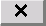
\includegraphics{button4rosemanual}} & The class will also be deleted from the \vdmpp{} model.\\ \hline
QuickSort          & \resizebox{1cm}{!}{
\includegraphics{button2rosemanual}} (default) & The class will be added to the \vdmpp{} model.\\
                   & \resizebox{1cm}{!}{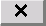
\includegraphics{button4rosemanual}} & The class will be excluded from both models.\\ \hline
SortMachine             & \resizebox{1cm}{!}{
\includegraphics{button3rosemanual}} (default)& No updates will be made, because the class has not been changed in either model.\\
                   & \resizebox{1cm}{!}{
\includegraphics{button1rosemanual}} & as the default action\\ 
                   & \resizebox{1cm}{!}{
\includegraphics{button2rosemanual}} & as the default action\\
                   & \resizebox{1cm}{!}{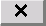
\includegraphics{button4rosemanual}} & The class will be excluded from both models.\\ \hline
\end{tabular}
\caption{Possible actions when merging the \vdmpp{} and the UML models\label{tab:actions}}
\end{center}
\end{figure}

\subsubsection*{Merging Classes with Conflicting Definitions}
\label{mergingclasses}
 
When the UML and \vdmpp{} models are allowed to evolve in parallel the
possibility of conflicts arise. If, for instance, both the \vdmpp{}
and UML model defines an operation with the same name but with
different signatures the Merge Tool will not know which one of the two
operations to choose for the resulting model. Clicking the ``Map''
button will start the merging of the two models, but if conflicts are
encountered, the merge will be aborted, and the user will be informed
about the classes with conflicts.

For example merging the \vdmpp{} and UML representations of the class
{\tt ExplSort} will cause conflicts, because the models differ in the
name of one of the arguments to the function {\tt RestSeq}. This
conflict is also evident in Figure~\ref{fig:diffs}.

The user will typically use the ``Diff'' button to locate the
conflict(s) and decide which one of the two definitions to keep,
simply by modifying the UML or \vdmpp{} model accordingly. When all
conflicts are resolved, the \vdmpp{} specification should be syntax
checked and the \link{} re-invoked to do the merging of the two
models.

Instead of modifying one of the models to avoid conflicts, the user
can also choose to change the mode of merging in order to solve the
conflict. Simply click the action button to toggle between the
different states and choose an action that suppresses one of the two
representations. Conflicts will only arise when representations are
merged!

\subsubsection*{Updating the \vdmpp{} Specification}
\label{updating}
  
If the \vdmpp{} and UML model are not in conflict with each other,
clicking the ``Map'' button will automatically update the class
repository of \rose{} to contain the result of merging the two
original models.  In the same way the {\tt rtf} files of the \vdmpp{}
project will automatically be updated and parsed to reflect the
changes made to the UML model. If new classes were introduced, they
will be generated as new {\tt rtf} files as described in
Section~\ref{trans2}.

Before updating an {\tt rtf} file the \link{} creates a copy of the
file. The copy is named by adding {\tt \_old.rtf} to the original file
name. I.e.\ the file {\tt ExplSort.rtf} will be copied to {\tt
  ExplSort.rtf\_old.rtf} before it is updated.

The following rules are applied when the \vdmpp{} specification files
are updated:
\begin{description}
\item[New elements] are added at the topmost position possible in the
  class.  For example, a new instance variable will be inserted at
  the top of the first {\tt instance variables} block of the class. If
  an {\tt instance variables} block was not already declared in the
  \vdmpp{} class, it will be generated at the topmost position of the
  class.
\item[Obsolete elements] will be removed from the file by converting
  them to \vdmpp{} comments. In this way unexpected removals can
  easily be restored.
\item[Modified elements] are handled by simply removing (by comments)
  the old definition and adding the new definition.
\end{description}
All modifications of the specification files will be identified by
comments like: ``Added by the Rose-VDM++ Link'' or ``Removed by the
Rose-VDM++ Link''.

Figure~\ref{fig:update} shows how the class {\tt ExplSort} was been
updated by the \link{} because the signature of the function {\tt
  RestSeq} had been modified in UML.

In some situations the \link{} will not be able to update the
necessary files.  Certain word processors lock the file(s) that is
currenly being edited such that other applications may not access
them. As a consequence the \link{} is unable to update such locked
files. If files that need to be updated are locked by another
application, the \link{} will list the names of these files, and the
user can then choose to either unlock these files (by making sure that
other applications are not using them) or cancel the merge process.

All files modified by the \link{} are subsequenty automatically parsed
so that the model contained in the \ToolboxName{} is identical to the
model contained in \rose{}.

\begin{figure}[htb]
\begin{center}
\mbox{}
\resizebox{11cm}{!}{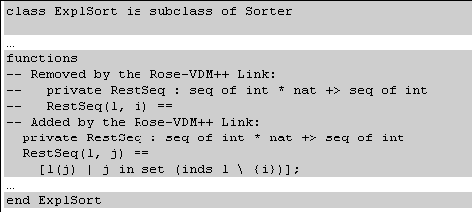
\includegraphics{updatedRtf}}
\caption{The updated {\tt ExplSort.rtf} file\label{fig:update}}
\end{center}
\end{figure}


\subsection{Type Checking of Specifications}
\label{sec:typecheck}

In order to use the \link\ the \vdmpp\ specification need only be
syntax checked, but it is recommended that it is type checked as well.
Information about relationships between classes defined by instance
variables is not available until the specification is type checked.
Therefore if a \vdmpp\ specification is only syntax checked it may not
be complete in the sense that the \link\ cannot generate association,
which are defined by such relations.

\newpage  
\section{Rational Rose}
\label{rose98}
  
So far we have discussed some of the features of the \link{}. Since
this tool relies on a very tight coupling with \rose{} it is within
the scope of this manual to give a short introduction to \rose{}.
Initially we will describe how to create class diagrams from the
classes generated by the \link{} or classes created by the user.
Section~\ref{manipulate} will describe how to modify, delete or add
any definitions in \rose{}.  

The \link{} is a so-called Language Add-In of \rose{}, which is
installed as described in~\cite{InstallPPMan-CSK}. The Add-In may be
activated or deactivated through the Add-In Manager of \rose{}.
Activating the \link{} (it is activated by default) makes \rose{}
aware of \vdmpp{}, the fundamental data types of \vdmpp{} and the
special stereotypes used by the mapping from UML to \vdmpp{}.

\subsection{Class Diagrams in Rational Rose}
\label{diagrams}
  
\subsubsection*{Creating Class Diagrams}

Translating \vdmpp{} class definitions to UML only creates or updates the class definitions   
in the class repository of \rose{} - it does not automatically create class diagrams. 
However \rose{} makes it easy to create class diagrams.
  
In order to create class diagrams in \rose{}, you should do as follows (note that   
the following actions are made from inside \rose{}):

\begin{enumerate}  
\item Either create an empty class diagram, or open an already existing one.  
\item Add classes to the class diagram by either 
\begin{itemize} 
\item Drag-and-drop: click a class in the class repository and drag it into the class   
diagram to which you wish to add it.  
\item Select {\it Query/Add Classes...}, and choose the package containing the classes   
you wish to add (this would typically be the "Generated classes" package).   
Move the classes to be added into the "Selected classes" list box, and click   
"OK". This will automatically add all selected classes to the currently active   
diagram, and automatically layout the diagram as well.  
\end{itemize}
\end{enumerate}

In Figure~\ref{fig:classdiagram} we show a class diagram created by following this approach.  

\begin{figure}[htb]
\begin{center}
\mbox{}
\resizebox{9cm}{!}{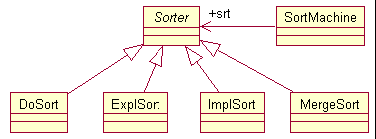
\includegraphics{classDiagram}}
\caption{The class diagram in \rose{} for the Sort example\label{fig:classdiagram}}
\end{center}
\end{figure}

\subsubsection*{Modifying Diagrams}

\rose{} also lets you change the   
layout of generated diagrams. Simply move the classes and relations to other   
classes as you like, by using the mouse.  
Modifying a class diagram in \rose{} has the following consequences:  
\begin{itemize}
\item Changing the layout, i.e., by moving classes and relations only modifies the   
diagrams, will have no consequence to the class repository. Furthermore, if the   
\link{} at a later time updates the repository, this will not alter the   
layout of the diagrams. Only if a class is removed from the repository, or if its   
relations to other classes are changed, this will change the appearance of the   
diagram. However, the layout will still be intact.  
\item Adding relations (either inheritance or association) between
  classes will change the class definition in the class repository,
  i.e.\ add the new relation to the model.  The diagram in which the
  new relation was added will naturally show the changes immediately.
  Other diagrams will, however, not show the new relation(s), but must
  be updated in order to reflect the changes. The next section
  describes how to update your class diagrams.
\item Changing the instance variables, operations, etc. of a class will immediately be   
visible in all other diagrams containing the class.  
\end{itemize}

\subsubsection*{Filtering Relationships}
  
\rose{} offers you the possibility to leave certain types of relations out of the currently   
selected diagram. Using this functionality you can easily construct a diagram showing   
only the inheritance relations between the classes in the diagram.   
In \rose{}, select {\it Query/Filter relationships...} in order to specify what kind of relations   
to display in the diagram. Figure~\ref{fig:relations} shows the dialogue box for filtering relations.  

\begin{figure}[htb]
\begin{center}
\mbox{}
\resizebox{7cm}{!}{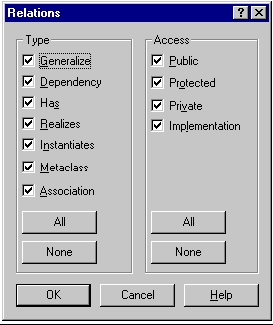
\includegraphics{relations}}
\caption{Specifying relations\label{fig:relations}}
\end{center}
\end{figure}

You can also use this dialogue box to update the relations of a
diagram. Simply select all possible kinds of relations (use the
``All'' button) and click ``OK''. This will re-display all relations
defined between the classes in the currently selected class diagram.
This is the only way to make new associations added by the \link{}
  visible in already existing diagrams.

\subsubsection*{Local Views}
Often one single class diagram, showing all classes and their mutual relations, will become too   
complicated, and consequently difficult to comprehend. For this reason  
\rose{} gives you the possibility to generate local views.

To do so, generate a new class diagram, which initially consists of one
or more classes, for which you want to generate a local view.  Select afterwards the
classes in this new diagram and choose the {\it Query/Expand Selected
  Elements...} menu item. A dialogue window will pop up allowing you
to determine the number of levels and the kind of relations you want
to see in the generated local view.
Clicking the ``OK'' button will now create a class diagram showing the generated local view.

Using this procedure you can for example easily generate a new class diagram
representing a class and all its immediate super- and sub classes.

\subsection{Manipulating Definitions in Rational Rose}
\label{manipulate}
  
At any time you are allowed to modify, delete or add any definitions in \rose{}. 
This section presents some examples of how to change your Rose model.

\subsubsection*{Modifying Definitions in the Repository}
  
The definition of attributes (i.e., instance variables and values
%and time variables
in \vdmpp{}) and operations (operations and functions
in \vdmpp{}) can easily be modified in \rose{}. Simply double-click
the class you wish to modify, and you are presented with a dialogue
box offering you to inspect and change the definition of every part of
the class.  The ``Class Specification'' window is used to browse the
specification of a given class. Figure~\ref{fig:classspecification}
shows the class specification window for the {\tt SortMachine} class.

\begin{figure}[htb]
\begin{center}
\mbox{}
\resizebox{7cm}{!}{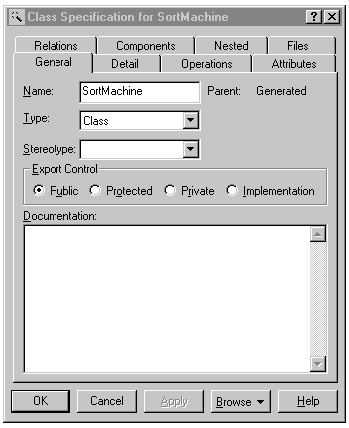
\includegraphics{sortMachineClass}}
\caption{UML Class Specification for the class {\tt SortMachine}\label{fig:classspecification}}
\end{center}
\end{figure}

\subsubsection*{Creating Certain Types of Entities}
  
Here we will describe how to create some new entities in \rose{}.  It
is recommended to read Section~\ref{mapping} in order to get some
information about the entities of UML, which can be mapped to \vdmpp{}
constructs. The \vdmpp{} add-in of \rose{} helps you when creating new
entities. In the following, we will describe the creation of classes,
attributes, operations and associations.

\begin{itemize}
\item{\bf Classes} 

A new class can be created by selecting the
  \resizebox{1cm}{!}{
\includegraphics{button5rosemanual}} button of
  \rose{}. To make use of the fundamental \vdmpp{} types and the
  predefined stereotypes defined by the \link{} a new class must be
  assigned to a \vdmpp{} component. To do so, follow these steps:
  \begin{itemize}
  \item Create a new component by right-clicking the ``Component
    View'' package in the browser of \rose{} and select {\em
      New/Component}. Double-click the new component, and in the
    specification window for this component (on the ``General'' tab)
    select \vdmpp{} as the language for this component.
  \item Select the ``Realizes'' tab in the specification window for
    the new component. Select the classes that should be assigned to
    this component. Right-click the selection and choose ``Assign''.
    Now these classes are assigned to the \vdmpp{} component.
  \end{itemize}
  Alternatively classes can be assigned to a particular component by
  simply ``dragging'' them into the component with the mouse.

\item{\bf Attributes}

  As described in Section~\ref{mapping} attributes in UML are used to
  represent instance variables and values
%   and time variables
of \vdmpp{}.
  A new attribute can easily be added to a class by right-clicking the
  class and selecting the menu item {\it New Attribute}.
  
  We use {\it stereotypes}, as described in Section~\ref{mapping}, to
  distinguish the three different \vdmpp{} constructs.  You can assign
  a stereotype (indicated by ``{\tt <<}'' ``{\tt >>}'') to each
  attribute.  If you do not specify a stereotype the attribute will be
  considered as an instance variable by default.
  
  The \vdmpp{} add-in helps you in defining stereotypes for
  attributes.  Figure~\ref{fig:stereotype} shows the ``Attribute
  Specification'' window of a newly added attribute.  Because the
  class is assigned to the \vdmpp{} component, one can choose between
  the three predefined stereotypes, {\tt <<instance variable>>} or {\tt
    <<value>>}.
%     or {\tt <<time variable>>}.


\begin{figure}[htb]
\begin{center}
\mbox{}
\resizebox{7cm}{!}{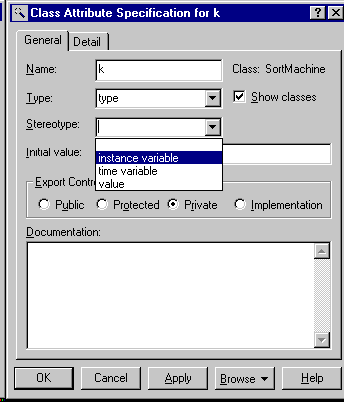
\includegraphics{stereotype}}
\caption{Selecting a predefined Stereotype for an Attribute.\label{fig:stereotype}}
\end{center}
\end{figure}

\item {\bf Operations}
  
  A new operation can easily be added to a class by right-clicking the
  class and selecting the menu item {\it New Operation}.

As with attributes, we use stereotypes to distinguish between
functions and operations of \vdmpp{}. These stereotypes are created as
with attributes. By default everything is considered as operations if the
stereotype is omitted.

\item{\bf Associations}
  
To create an association between two classes, simply click the ``Association Tool'' and   
define the association by clicking one class and dragging the mouse to the other class.   
You can specify further details for the association by double clicking it, which will open   
the ``Association Specification'' window. Here you can add role names, cardinalities and   
constraints to the association.  


\begin{description}
\item [Role names:] As described in the mapping rules the role name of an association is used as   
a name for the instance variable the association will be translated to. For this reason,   
giving an association at least one role name is vital for it to appear as an instance   
variable in the generated \vdmpp{} class. If no role names are specified for an association it   
will simply be ignored.  
\item [Cardinality:] If no cardinality is specified for a role a cardinality of one is assumed as   
default.  
\item [Constraints:] In the ``Association Specification'' window it is
  possible to add constraints to the role of an association. This
  can be used to add a constraint like {\tt \{ordered\}} to a role,
  which would generate a {\it sequence}, rather than a {\it set} of
  object references when translated to \vdmpp{}.
\item [Qualifiers:] A qualifier can easily be added to an association.
  Simply right-click the association close to the class to hold the
  qualifier and then select {\em New Key/Qualifier}. Specify as name of
  the qualifier the \vdmpp{} type to be used as domain in the map used
  to model qualified associations in \vdmpp{} (see
  Section~\ref{mapping}).  Notice that right-clicking the association
  near the role to be modified can modify many details of the two
  roles of an association.
\end{description}  
\end{itemize}
  
\newpage  
\section{Mapping Rules between VDM++ and UML}
\label{mapping}
  
In this section we present the relation between \vdmpp{} and UML. That is, we present the   
rules applied by the \link{} when translating one representation into the other.  

Clearly, to fully understand the following mapping rules, a detailed knowledge of \vdmpp{}   
and UML is required. Here we will not introduce the two notations, but merely describe   
various constructs whenever necessary. We refer to \cite{LangManPP-CSK} and \cite{Booch&97} for a   
complete presentation.  
The rules presented in the following section are summarised in Figure~\ref{tab:mapping} in appendix~\ref{rules}.  

The rules will be presented by presenting several \vdmpp{}
specifications along with their corresponding UML translation. In this
regard it is important to mention that the defined mapping is {\it
  injective}, i.e., by defining the mapping from \vdmpp{} to UML, we
have defined the inverse mapping at the same time.
 
Furthermore, it is important to note that the following rules do {\it not} cover every construct   
possible to write in \vdmpp{}, nor do they cover every aspect of the UML. The mapping   
rules have simply been defined in order to make the mapping injective, meaning that   
constructs that can only be described in one of the two representations are left out of the   
mapping.  

The \link{} will simply ignore constructs not covered by the following   
mapping rules.  

\subsection{The Class Structure}
\label{classstructure}
  
This section covers how the internal class structure is being mapped between the two   
representations. Each subsection addresses various \vdmpp{} constructs.  

\subsubsection*{Instance Variables and Values}
  
In \vdmpp{} the internal state of an object is described by its instance variables and its value   
definitions. The main difference between values and instance variables is that values are   
read-only. In UML the internal state is described in the attribute section in which we will   
simply list the instance variables and values along with their corresponding types and   
value. In order to distinguish instance variables and values we will use two {\it stereotypes},   
namely {\tt <<instance variable>>} and {\tt <<value>>}.  

The syntax for declaring attributes in UML is:  

\begin{quote}
\begin{verbatim}
name : type = initial-value
\end{verbatim}
\end{quote}

which is almost identical to the syntax of instance varaible and value
definitions in \vdmpp{}. Consequently values and instance varaibles
can be mapped directly to UML.  Figure~\ref{fig:queue} illustrates the mapping of
instance variables and values.

%\subsubsection*{Time Variables}  
%
%In \vdmpp{} real-time behaviour can be expressed through the use of time variables to   
%represent continuous functions of time. Time variables can be either input or output   
%variables, distinguished in \vdmpp{} by the optional keyword {\tt input}. At the UML level time   
%variables will be listed as attributes and distinguished from values and instance variables   
%by the stereotype {\tt <<time variable>>}. In UML adding the constraint {\tt \{input\}} to the   
%name of the time variable will identify input time variables.  
%Time variables can be subject to invariants in the same way as instance variables are, only   
%here expressed as either {\it assumptions} or {\it effects}. Assumptions apply to input variables and   
%describe the requirements the input must fulfil for the system to function properly (i.e., an   
%invariant on input variables), while effects describe the expected behaviour of output   
%variables. The mapping, however, will not consider neither the assumptions nor the effect   
%clauses.  

\begin{figure}[htb]
\begin{center}
\hspace{-2cm}
\begin{minipage}[t]{2.5in}
\verbatimfile{class.vpp}
\end{minipage} \ \
\begin{minipage}[t]{2in}
\vspace{2cm}
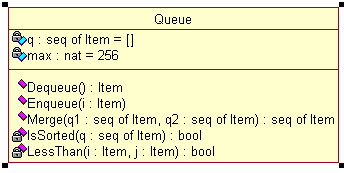
\includegraphics[width=2.8in]{queueClass}
\end{minipage}
\caption{Mapping a class between \vdmpp{} and UML\label{fig:queue}}
\end{center}
\end{figure}

\subsubsection*{Operations and Functions}
  
Operations and functions map into the operations section of the UML
class. They are distinguished by the stereotypes {\tt <<operation>>}
and {\tt <<function>>}. The syntax for defining operation headers in
UML is:

\begin{quote}
\begin{verbatim}
name(parameter : type, ...) : return-type  
\end{verbatim}
\end{quote}
  
which is almost identical to the syntax for implicitly defined
functions/operations in \vdmpp{}.

Explicitly and implicitly defined function headers, as well as
operation headers must be transformed into this syntax. See
Figure~\ref{fig:queue} for an example of mapping operations and
functions. 

Pre and post conditions defined in operations are preserved by the UML
mapper. Thus they need to be written as syntactically correct VDM
expressions. Since UML does not provide any way of defining a result
identifier for an operation, the special identifier \textbf{RESULT}
should be used in post conditions to represent the result of the
operation. 

Mapping explicit and implicit functions into the same syntax in UML
makes it difficult to distinguish between implicitly and explicitly
defined functions when mapping from UML to \vdmpp{}. For this reason,
the following rules are applied when mapping functions from UML to
\vdmpp{}:

\begin{itemize}
\item If a function is already defined in \vdmpp{}, it is mapped into
  the same kind (implicit or explicit) as defined in \vdmpp{}.
\item If a function is not known in \vdmpp{} (i.e., the function was
  defined at the UML level) it is mapped as explicit.
\end{itemize}

\subsection{Associations between Classes}
\label{assoclasses}
  
In \vdmpp{} an object (an instance of a class) may have relations to
objects of other classes or objects of its own class. Such clientship
relations are possible through the object reference type. In UML such
relations are called associations and represented by an arrow from the
{\it client} class towards the class being referenced. In this way the
arrow indicates the {\it navigability} of the \link{}, i.e., which
object can in fact be referenced by the other. Figure~\ref{fig:classA}
shows how such simple associations are mapped between \vdmpp{} and
UML. Notice, that the instance variables representing the object
references are not shown as attributes in the UML class.

\begin{figure}[htb]
\begin{center}
\hspace{-2cm}
\begin{minipage}[t]{2in}
\begin{verbatim}
class A  
instance variables  
  a: A;  
  b: B;  
  c: C;  
end A  
  
class B  
end B  
  
class C  
instance variables  
  a: A;  
end C  
\end{verbatim}
\end{minipage} \ \
\begin{minipage}[t]{2in}
\vspace{1cm}
\resizebox{8cm}{!}{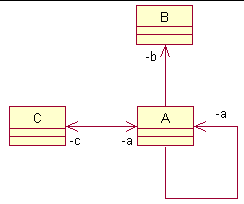
\includegraphics{refs}}
\end{minipage}
\caption{Mapping object references/associations between \vdmpp{} and UML\label{fig:classA}}
\end{center}
\end{figure}


\renewcommand{\textfraction}{0}
                              

\renewcommand{\topfraction}{1}
                              

\setcounter{totalnumber}{100} 
\setcounter{topnumber}{100} 
   
In UML the {\it far end} of an association is called a role. Usually
roles are given names which, at least in real world models, tend to
{\em describe} the role of the association. Roles are particular
helpful in the case of binary associations. Here we will construct
role names simply from the name of the instance variable representing
the association. This is also shown in Figure~\ref{fig:classA}.

\subsubsection*{Adding Multiplicity to Associations}
  
So far we have only considered simple ``one-to-one'' associations, i.e., relations   
connecting one instance of a class with exactly one other instance.  By using constructs   
like {\tt seq of A} and {\tt set of A}, it is possible to relate one instance to several other   
instances. In UML multiplicity is represented by adding numbers/symbols to the ends of   
associations, thereby indicating the multiplicity.  

We will now present how different \vdmpp{} constructs related to multiplicity of   
associations are mapped to UML.  

\begin{description}
\item [{\tt set of objref}:]  This construct is translated into a ``one-to-many'' association, which in   
UML is modelled by placing a ``1'' at the one-end, and the range ``0..*'' at the many-  
end of the association.  
\item [{\tt seq of objref}:]  This is also a one-to-many association, but using the sequence type adds   
an ordering to the references, which in UML is indicated by adding the {ordered}   
constraint to the many-end of the association.  
\item [{\tt seq1 of objref}:]  The non empty sequence of object references is represented by the   
range ``1..*'' at the many-end of the association.  
\item [{\tt [objref]}:]  The optional object reference will be identified by adding the range ``0..1'' to   
the role of the association.  
\end{description}

These constructs are summarised in Figure~\ref{fig:classD}. 

\begin{figure}[htb]
\begin{center}
\hspace{-2cm}\begin{minipage}[t]{2in}
\begin{verbatim}
class D  
instance variables  
  es: set of E;  
  fs: seq1 of F;  
end D  
  
class E  
instance variables  
  opt_f: [F];  
end E  
  
class F  
instance variables  
  d: D;  
end F  
\end{verbatim}
\end{minipage} \ \
\begin{minipage}[t]{2in}
\vspace{1cm}
\resizebox{8cm}{!}{\includegraphics{multiRefs}}
\end{minipage}
\caption{Mapping multiple object references between \vdmpp{} and UML\label{fig:classD}}
\end{center}
\end{figure}

\subsubsection*{Object References using {\tt map} and {\tt inmap}}
In \vdmpp{} it is possible to relate objects using the map and inmap
type. \vdmpp{} constructs like: {\tt map type to objref}, where {\tt
  type} can be any \vdmpp{} type and {\tt objref} is a simple or
multiple object reference will result in a {\it qualified
  association}.

The multiplicity of qualified   
associations is added as with the other types of associations. In UML the qualifier   
itself can be assigned a name, which in this case will be the type of the domain of the   
map. As with other associations the role name of the association is the name of the   
instance variable representing the map. See Figure~\ref{fig:classG} for an example. 

\begin{figure}[htb]
\begin{center}
\hspace{-1cm}
\begin{minipage}[t]{2.5in}
\begin{verbatim}  
class G  
instance variables  
  qual_h: map nat to H;  
end G  
  
class H  
instance variables  
  qual_j: map real to J;  
end H  
  
class J  
instance variables  
  qual_h: map nat to set of H;  
end J  
\end{verbatim}
\end{minipage} \ \
\begin{minipage}[t]{2.5in}
\vspace{1cm}
\resizebox{7cm}{!}{\includegraphics{qualifiedAssociations}}
\end{minipage}
\caption{Qualified associations from object references defined using maps\label{fig:classG}}
\end{center}
\end{figure}

\begin{figure}[h]
\vspace{1cm}
\begin{center}
%\hspace{-2cm}
\begin{minipage}[h]{2.5in}
\begin{verbatim}  
class Super  
operations
  methodA() ==  
    is subclass responsibility;  
  methodB() ==  
    ...;  
end Super  
  
class SubA is subclass of Super  
end SubA  
  
class SubB is subclass of Super  
end SubB  
\end{verbatim}
\end{minipage} \ \
\hspace{1cm}
\begin{minipage}[h]{2.5in}
\vspace{1cm}
\resizebox{6cm}{!}{\includegraphics{inheritance}}
\end{minipage}
\caption{Mapping inheritance between \vdmpp{} and UML\label{fig:super}}
\end{center}
\end{figure}

\subsubsection*{Inheritance Relationship}
\label{inheritance}

The translation of inheritance from \vdmpp{} to UML and vice versa is
straightforward.  Figure~\ref{fig:super} shows an example. The class
{\tt SubA} and the class {\tt SubB} inherit from class {\tt Super}.
In UML, inheritance relationships are shown as generalisations.
  
\subsubsection*{Delegation}

In \vdmpp{} the specification of operations can be delegated to
subclasses by using the {\tt is subclass responsibility} clause. In
UML such operations are called {\it abstract operations}, and classes
containing abstract operations are called {\it abstract classes}, as
opposed to concrete classes.  A class will be considered abstract, if
it delegates at least one of its operations (i.e., at least one operation is
specified using {\tt is subclass responsibility}), otherwise it is
considered concrete. In UML abstract classes and operations are
identified by writing their names in Italics font.


\bibliographystyle{iptes}
\newpage
\bibliography{ifad}  
  
\newpage
\appendix
\section{Summarising the Mapping Rules}
\label{rules}
The table in Figure~\ref{tab:mapping} summarises the mapping rules applied by the \link{}:  
\begin{figure}[!hb]
\begin{center}
\mbox{}
\begin{tabular}{|p{65mm}|p{8cm}|} \hline
  \vdmpp{}           & UML  \\ \hline \hline
  instance variable            & attribute with stereotype {\tt <<instance variable>>} \\ \hline
   value          & attribute with stereotype {\tt <<value>>}\\ \hline
%   time variable          & attribute with stereotype {\tt <<time variable>>}. Input time variables are marked by the   
%constraint {\tt \{input\}}  \\ \hline
 operation           & operation with stereotype {\tt <<operation>>} \\ \hline
  function          & operation with stereotype {\tt <<function>>}. Functions, that are only defined in UML are mapped to   
\vdmpp{} as explicit functions. Otherwise   
functions are mapped implicit or explicit as   
defined in \vdmpp{}.   \\ \hline
  {\tt obj: OtherClass}            & \resizebox{7.9cm}{!}{\includegraphics{thisclass1}} \\ \hline
  {\tt obj: set of OtherClass}         & \resizebox{7.9cm}{!}{\includegraphics{thisclass2}} \\ \hline
  {\tt obj: seq of OtherClass}        & \resizebox{7.9cm}{!}{\includegraphics{thisclass3}} \\ \hline
  {\tt obj: seq1 of OtherClass}         & \resizebox{7.9cm}{!}{\includegraphics{thisclass4}} \\ \hline
  {\tt obj: [OtherClass]}         & \resizebox{7.9cm}{!}{\includegraphics{thisclass5}} \\ \hline
  {\tt obj: map type to OtherClass}         & \resizebox{7.9cm}{!}{\includegraphics{thisclass6}} \\ \hline
  {\tt class ThisClass is subclass}\newline {\tt of OtherClass}   & \resizebox{2.5cm}{!}{\includegraphics{thisclass7}} \\ \hline
\end{tabular}
\caption{Mapping rules applied by the \link{}\label{tab:mapping}}
\end{center}
\end{figure}

\clearpage

\section{Warnings generated by the Rose-VDM++ Link}
\label{warnings}

Review Figure~\ref{fig:architecture}. Before merging the two models,
both the \vdmpp{} and the UML models are translated to an internal
representation.

This translation involves some checks, which can lead to different
warnings.
%%
%% For the time being these warnings are NOT generated:
%%
%% \subsubsection*{Warnings Generated during the Translation from \vdmpp{}  to UML}
%%   
%% During the translation from \vdmpp{} to UML certain warnings may be
%% generated. As mentioned earlier, the mapping rules described in
%% Section~\ref{mapping} define how one representation is translated into
%% the other. However, if one writes a \vdmpp{} construct, which does not
%% "fit" into the defined mapping rules, the user will be notified by a
%% warning identifying the \vdmpp{} construct causing the warning.
%% 
%% The \vdmpp{} constructs causing the warnings are 
%% instance variables which are defined somehow using the object reference
%% type, but which do not ``fit'' into the
%% defined mapping rules.
%% 
%% These instance variables will be mapped to UML simply as instance variables
%% and not as associations.
%% 
%% Look at the following example:
%% 
%% \begin{quote}
%% \begin{verbatim}
%% class ThisClass
%% 
%% instance variables
%% 
%%   obj: set of seq of OtherClass
%% 
%% end ThisClass
%% 
%% class OtherClass
%% end OtherClass
%% \end{verbatim}
%% \end{quote}
%% 
%% The loading of the \vdmpp{} model will result in a warning, which can
%% be seen in Figure~\ref{fig:warningThisClass}.  Moreover, mapping the
%% \vdmpp{} specification to UML without removing the construct causing
%% the warning, will result in the UML model, shown in
%% Figure~\ref{fig:wrongUML}.
%% 
%% \begin{figure}[htb]
%% \begin{center}
%% \mbox{}
%% \vspace{0.5cm}
%% \resizebox{6cm}{!}{\includegraphics{fig18rosemanual}}
%% \caption{Warning generated when computing a UML representation for the instance variable {\tt set of seq of OtherClass}.\label{fig:warningThisClass}}
%% \end{center}
%% \end{figure}
%% 
%% \begin{figure}[htb]
%% \begin{center}
%% \mbox{}
%% \vspace{0.5cm}
%% \resizebox{6cm}{!}{\includegraphics{fig19rosemanual}}
%% \caption{The generated UML model.\label{fig:wrongUML}}
%% \end{center}
%% \end{figure}

\subsubsection*{Warnings Generated during the Translation from UML to \vdmpp{}}

When a UML class is translated to \vdmpp{}, the UML attributes and
operations are converted to \vdmpp{} constructs.  The name and types
used in the UML model must consequently comply with the syntactical
rules of \vdmpp{}. If this is not the case, the UML definition is
simply ignored and the user is notified by a warning.  This is done in
order to maximise the syntactical correctness of the \vdmpp{}
specification generated.

As an example look at the UML class shown in Figure~\ref{fig:noncompliance}.

\begin{figure}[htb]
\begin{center}
\mbox{}
\vspace{0.5cm}
\includegraphics{noncompliance}
\caption{UML class that does not comply with the syntax 
rules of \vdmpp{} (the \$\ sign cannot be used here)\label{fig:noncompliance}}
\end{center}
\end{figure}

The generated warning when loading the UML model is shown in Figure ~\ref{fig:warning}.
\begin{figure}[htb]
\begin{center}
\mbox{}
\vspace{0.5cm}
\resizebox{9cm}{!}{\includegraphics{warning}}
\caption{The warning generated if the definition of an instance
  variable does not comply to the syntactical rules of \vdmpp{}\label{fig:warning}}
\end{center}
\end{figure}
Mapping the UML model to \vdmpp{} without removing the UML definition
causing the warning will result in the following \vdmpp{} class
definition:

\begin{quote}
\begin{verbatim}
class ThisClass
end ThisClass
\end{verbatim}
\end{quote}

As you can see, the generated class definition is simply empty.
\end{document}





